\section{Exercise 1}

As part of your job as a security analyst, one of your clients discovers that their network is compromised. 
In particular, from an early analysis, they have ground to suspect that the start of the compromise was a network attack against the computer of the administrative assistant.

Consider the following (simplified) schema of the company network.
\begin{figure}[H]
    \centering
    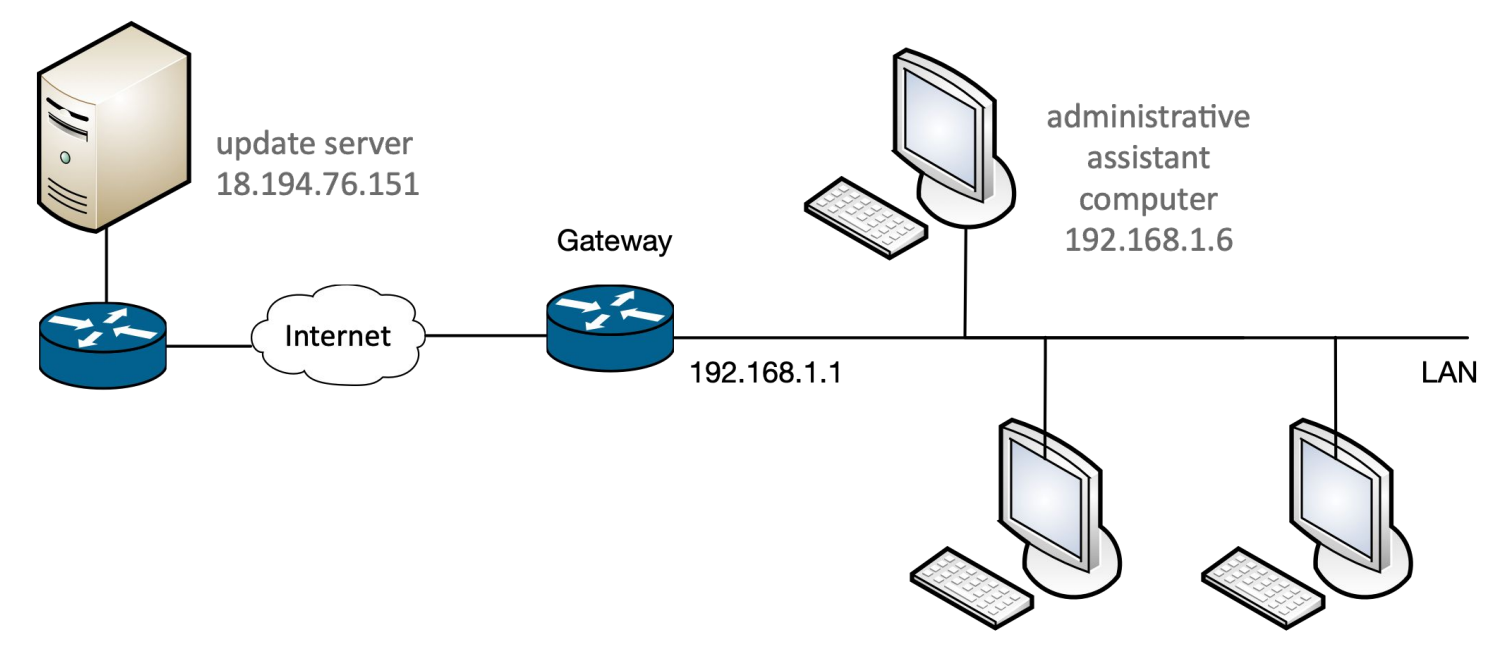
\includegraphics[width=0.75\linewidth]{images/net.png}
\end{figure}
Your client managed to capture the network traffic on the administrative assistant's computer (IP address 192.168.1.6 and MAC address dc:a9:04:7a:ce:29) when the attack was taking place. 
During the traffic capture, the computer was automatically updating a well-known accounting software from the software vendor's web server (IP address 18.194.76.151 and MAC address dc:a6:03:01:02:fe). 
You also know that the IP address of the LAN interface of the company's network gateway is 192.168.1.1, and its MAC address is b6:28:97:ca:b7:48.
\begin{itemize}
    \item dc:a9:04:7a:ce:29 $\rightarrow$ ff:ff:ff:ff:ff:ff ARP Who has 192.168.1.1? Tell 192.168.1.6
    \item 38:60:77:b9:79:98 $\rightarrow$ dc:a9:04:7a:ce:29 ARP 192.168.1.1 is at 38:60:77:b9:79:98
    \item b6:28:97:ca:b7:48 $\rightarrow$ dc:a9:04:7a:ce:29 ARP 192.168.1.1 is at b6:28:97:ca:b7:48
    \item 192.168.1.6 (dc:a9:04:7a:ce:29) $\rightarrow$ 18.194.76.151 (38:60:77:b9:79:98) TCP SYN
    \item 18.194.76.151 (38:60:77:b9:79:98) $\rightarrow$ 192.168.1.6 (dc:a9:04:7a:ce:29) TCP SYN, ACK
    \item 38:60:77:b9:79:98 $\rightarrow$ dc:a9:04:7a:ce:29 ARP 192.168.1.1 is at 38:60:77:b9:79:98
    \item 192.168.1.6 (dc:a9:04:7a:ce:29) $\rightarrow$ 18.194.76.151 (38:60:77:b9:79:98) TCP ACK
    \item 38:60:77:b9:79:98 $\rightarrow$ dc:a9:04:7a:ce:29 ARP 192.168.1.1 is at 38:60:77:b9:79:98
    \item 192.168.1.6 (dc:a9:04:7a:ce:29) $\rightarrow$ 18.194.76.151 (38:60:77:b9:79:98) TCP HTTP GET /downloads/software-update.exe
    \item 18.194.76.151 (38:60:77:b9:79:98) $\rightarrow$ 192.168.1.6 (dc:a9:04:7a:ce:29) TCP HTTP 200 OK ...
\end{itemize}
\begin{enumerate}
    \item Describe the attack going on in the network, specifying the name and providing a short explanation of how the attack works in general.
    \item What is the goal of the attack, in this specific case? Motivate your answer.
    \item Can you tell the IP address of the attacker? And the MAC address?
    \item Given only the above packet capture, can you tell whether the attacker is located (i.e., on the LAN, on the same network of the web server, or on an arbitrary Internet-connected network)? Why?
\end{enumerate}

\subsection*{Solution}
\begin{enumerate}
    \item The attack is an ARP spoofing. 
        It is a type of attack in which a malicious actor sends falsified ARP (Address Resolution Protocol) messages over a LAN.
    \item Sniffing or manipulation of the traffic to or from the compromised machine. 
        We can rule out DOS as the traffic passes (there are responses from the server).
        Likely, given the scenario (malware infection), the attack is targeted at tampering with the data in transit rather than (or in addition to) sniffing.
    \item We cannot tell the real IP of the attacker, but the MAC is 38:60:77:b9:79:98 (that could be also spoofed).
    \item The attacker is located on the same network of the target machine, i.e., on the LAN. 
\end{enumerate}